\documentclass[11pt]{article}
\usepackage[margin=0.9in]{geometry}
\usepackage[T1]{fontenc}
\usepackage{lmodern}
\usepackage{amsmath,amssymb,array,booktabs,longtable}
\usepackage{enumitem,microtype}
\usepackage[obeyspaces,spaces]{xurl}
\usepackage[dvipsnames]{xcolor}
\usepackage{tikz}
\usetikzlibrary{arrows.meta,positioning}
\usepackage{fancyhdr}
\usepackage[hidelinks]{hyperref}
\setlist[itemize]{leftmargin=1.5em,itemsep=0.2em}
\setlist[enumerate]{leftmargin=1.7em,itemsep=0.3em}
\renewcommand{\arraystretch}{1.16}
\newcolumntype{L}[1]{>{\raggedright\arraybackslash}p{#1}}
\setlength{\LTpre}{0.7em}
\setlength{\LTpost}{0.7em}
\emergencystretch=5em
\DeclareUrlCommand{\code}{\urlstyle{tt}}
\newcommand{\filepath}[1]{\path{#1}}
\newcommand{\dossiertitle}{ProofSphere Exploit Proofs}
\newcommand{\dossiersubtitle}{Technical Design Dossier}
\newcommand{\dossierauthor}{Prepared by Codex}
\newcommand{\initialtimestamp}{Sunday, 11 October 2026, 14:57:00 EDT (-0400)}
\newcommand{\preparedtimestamp}{Sunday, 11 October 2026, 15:29:50 EDT (-0400)}
\definecolor{Ink}{HTML}{213B52}
\hypersetup{pdftitle={\dossiertitle},pdfauthor={\dossierauthor},
  pdfsubject={A bounded hackathon design for confidential exploit verification}}
\pagestyle{fancy}
\fancyhf{}
\fancyhead[L]{\small\dossiertitle}
\fancyhead[R]{\small Design baseline v0.2}
\fancyfoot[C]{\thepage}
\setlength{\headheight}{15pt}
\setcounter{tocdepth}{1}
\title{\dossiertitle\\[0.35em]\large\dossiersubtitle}
\author{\dossierauthor}
\date{Prepared \preparedtimestamp}

\begin{document}
\maketitle
\begin{center}
\begin{tabular}{L{0.21\linewidth}L{0.69\linewidth}}
\textbf{Workspace} & \filepath{/Users/light/Documents/proofsphere} \\
\textbf{Status} & Reviewed baseline v0.2; implementation not started \\
\textbf{Scope} & One synthetic vault, private calldata, genuine local proof, independent verification \\
\textbf{Canonical source} & \filepath{docs/proofsphere-hackathon-technical-design-dossier.tex} \\
\textbf{Companion} & Same basename with the \code{.pdf} extension \\
\textbf{Authority} & User-approved hackathon concept, simplified to omit severity scoring \\
\end{tabular}
\end{center}

\begin{abstract}
ProofSphere is a prototype for demonstrating an exploitable security property without transmitting the triggering transaction payload to the verifier. The selected demonstration uses a deliberately vulnerable Solidity vault with a fixed, synthetic initial state. A researcher executes a private transaction inside a zero-knowledge virtual machine and proves that an account with no deposit credit gains funds while the vault becomes undercollateralized and the victim's claim remains unchanged. An independent verifier accepts only a genuine proof bound to its expected guest program, registered scenario, and challenge. The first version returns a Boolean impact claim; it excludes severity scoring, bounty payments, arbitrary target uploads, and live-chain execution. This dossier defines the trust boundary, exact execution relation, artifact formats, ownership, implementation sequence, and acceptance gates. Repository inspection found no implementation, tests, or project tooling. External source inspection supports the architecture but does not establish local build compatibility, proof-generation cost, or cryptographic correctness of a future implementation. Those are explicit implementation gates.
\end{abstract}
\clearpage
\tableofcontents
\clearpage

\section{Purpose and Decision Authority}
This document is the implementation baseline for a bounded hackathon demonstration. It enables an engineer to construct the target, implement the proof statement, build a verifier, and distinguish a complete demonstration from a simulated interface. Normative requirements use \emph{must}; proposed file paths refer to work that does not yet exist. Creating this dossier authorizes the documentation deliverable only. It does not record that contracts, a prover, a portal, or deployments have been implemented.

The initial concept combined confidential exploit evidence with severity disclosure. The user's subsequent instruction permits a simpler design and questions the value of severity in the first version. The selected revision therefore removes severity classes, scoring, percentage thresholds, and maximum-damage claims. The retained product question is: \emph{can an ordinary account demonstrate unauthorized withdrawal without sending the owner its triggering payload?}

\begin{longtable}{L{0.19\linewidth}L{0.37\linewidth}L{0.34\linewidth}}
\toprule
\textbf{Decision} & \textbf{Selected behavior} & \textbf{Consequence} \\
\midrule
\endhead
Claim & Prove one unauthorized-withdrawal predicate. & No severity engine or CVSS interpretation. \\
Target & One vault family, vulnerable and patched variants. & No arbitrary application execution. \\
Witness & One private calldata byte string. & No private helper contract, multi-transaction program, or uploaded exploit source. \\
Execution & One direct, zero-value transaction from a fixed ordinary account. & No credentials, attacker capital, remote RPC, or deployment procedure in the witness. \\
Proof & Local RISC Zero succinct receipt. & No remote prover receives the witness. \\
Verification & Trusted guest identity plus trusted scenario and challenge. & A proof cannot select its own verification authority. \\
Demonstration & Genuine proof; live verification may use a clearly identified recorded artifact. & Generation may be precomputed; verification cannot be simulated. \\
\bottomrule
\end{longtable}

\section{Current Status and Evidence Base}
\subsection{Observed Repository State}
At initial preparation, \code{ls -la} showed only \code{.git}; \code{git status --short --branch} reported \code{No commits yet on master}. No README, source files, tests, dependency manifest, documentation convention, or local AGENTS file was found. The final review rechecked the same unborn branch and found only the untracked \filepath{docs/} deliverables. There is no existing implementation or compatibility contract to preserve. \filepath{docs/} remains the canonical dossier location.

The local machine exposes LaTeX and Poppler tools for artifact rendering. Node reports version 22.23.1, and the bundled pnpm executable reports 11.25.0. Rust's active default reports 1.83.0; an explicit 1.97.0 toolchain is installed. The inspection did not find \code{forge}, \code{rzup}, or \code{cargo-risczero} on the shell path. No SDK installation or implementation build was attempted. The available host toolchain does not imply that the RISC-V guest toolchain or prover assets are installed.

\subsection{External Source Inspection}
\begin{longtable}{L{0.23\linewidth}L{0.34\linewidth}L{0.33\linewidth}}
\toprule
\textbf{Source} & \textbf{Observed fact} & \textbf{Design implication} \\
\midrule
\endhead
\code{ziemen4/zkpoex}, commit \code{cdbb4facb8a5b6c18a536656773e324766253ee3} \cite{zkpoex} & Rust guest executes an EVM runner and commits a Boolean result with specification/context hashes. & EVM execution in a zkVM is an existing prototype architecture, not a new cryptographic primitive. \\
Same repository: guest, host, runner, and Justfile \cite{upstreamguest,upstreamhost,upstreamrunner,upstreamjust} & Declares RISC Zero 2.x and \code{evm} 0.42.0; runner selects Cancun; development mode defaults to 1 in its Justfile. & Use as inspected reference material. Do not copy its host, logging, environment handling, or defaults as the verification authority. \\
RISC Zero v3.0.6, commit \code{1cc70cf05033a79ebc90f07c679cb4bd1cd301b9} \cite{risc0receipt,risc0prover} & Receipts bind execution to an expected image ID and journal. Source exposes succinct proving and explicit development-mode controls. & Select a pinned SDK and reject nonproduction receipt types independently of environment settings. \\
Solidity 0.8.26 compiler documentation \cite{solidity} & Compiler supports standard JSON, deployed runtime output, storage layout, and an explicit EVM target. & Generate reproducible runtime bytecode and confirm the ledger slot; match the runner's Cancun configuration. \\
\code{evm} 0.42.0 documentation \cite{evm} & Rust EVM with memory backend and stack executor interfaces. & Select this inspected interpreter family for the narrow fixture; differential tests remain necessary. \\
\bottomrule
\end{longtable}

No external prototype was compiled or executed during preparation. No prover, network, smart-contract, or end-to-end implementation tests were run in this workspace. Source references establish inspected design interfaces, not operational readiness. Future evidence must include dependency locks, generated image ID, target hashes, test outputs, and real receipts.

\subsection{Implementation Readiness Review}
The final review retained the one-claim scope and corrected the following gaps. These are resolved design decisions, not completed implementation checks.
\begin{longtable}{L{0.25\linewidth}L{0.65\linewidth}}
\toprule
\textbf{Review finding} & \textbf{Revision and required implementation evidence} \\
\midrule
\endhead
Incomplete environment binding & Commit the interpreter's explicit post-Merge randomness value, including its presence tag; test changes independently. \\
Ambiguous state application & Specify transaction entry, nonce behavior, executor deconstruction, and backend application; compare observable contract behavior with Foundry. \\
Prover selection defaults & Construct the in-process local prover with explicit SDK features. Reject remote-selection settings and verify a genuine receipt in release mode. \\
Unspecified exchange files & Define exact public JSON fields, byte encodings, bounded guest input, recorded-mode startup, and request-generation behavior. \\
Private execution diagnostics & Retain proving cycles, time, memory, and intermediates locally; public reports contain only receipt identities and verifier measurements. \\
Implementation sequencing & Produce a genuine vault proof and an independent CLI result before portal work. A minimal arithmetic receipt establishes tooling only. \\
\bottomrule
\end{longtable}
The remaining feasibility question is whether the pinned EVM/zkVM combination can produce the real vault receipt on the chosen machine. The proof gate closes that question; additional product features do not.

\section{Glossary}
\begin{longtable}{L{0.22\linewidth}L{0.68\linewidth}}
\toprule
\textbf{Term} & \textbf{Meaning in this dossier} \\
\midrule
\endhead
Witness & Private calldata known to the researcher and supplied to local proof generation. \\
Statement & The public assertion that a qualifying transaction exists for a specific registered scenario and challenge. \\
zkVM & A virtual machine that produces a cryptographic proof of execution of its guest program. \\
Guest & The program whose execution is proved; it reconstructs the scenario, runs the EVM, and checks the impact predicate. \\
Image ID & Cryptographic identity of the compiled guest executable. The verifier chooses the expected value independently. \\
Receipt & SDK proof object containing a seal and public journal. A development receipt is not cryptographic evidence. \\
Journal & Exact public bytes committed by successful guest execution. It excludes calldata and execution traces. \\
Scenario & Owner-approved code, initial account/storage state, environment, and claim definition. \\
Challenge & Owner-generated random nonce binding a receipt to a particular request. It does not authenticate authorship. \\
Ledger credit & The vault's recorded amount owed to an account. It differs from the vault's actual native-currency balance. \\
Synthetic wei & Integer accounting unit with the same scale as Ethereum wei, used only in the local fixture. \\
\bottomrule
\end{longtable}

\section{Problem Diagnosis and Product Definition}
A conventional exploit report transmits enough detail for the recipient to reproduce the exploit. ProofSphere separates evidence of a defined outcome from disclosure of the input that causes it. The verifier must learn that the agreed claim is satisfied, without receiving the payload through the proof, portal, logging, or infrastructure.

The central engineering risk is a \emph{valid proof of the wrong computation}. A receipt is inadequate if the researcher can replace the target, fabricate initial balances, change the sender, choose a permissive claim, or direct verification to a different guest. These are binding and ownership failures. They must be resolved in the guest and independent verifier before interface work is promoted.

The product is a local workflow with three actions: obtain a registered challenge, generate a proof using a private local file, and verify the resulting artifact. The accepted result is \emph{Unauthorized withdrawal demonstrated}. The interface also identifies the target version and synthetic scenario. It presents no severity badge, guessed monetary maximum, or claim that a rejected report proves safety.

\subsection{Goals}
\begin{itemize}
\item Demonstrate one genuine exploit proof against fixed runtime bytecode and initial state.
\item Verify the artifact in a separate process without access to the witness or prover directory.
\item Bind acceptance to the verifier's expected image ID, scenario digest, challenge nonce, and impact claim.
\item Show corrupted artifacts and mismatched target/challenge identities being rejected.
\item Show the reference payload failing the same impact predicate against the patched variant.
\item Preserve a small implementation with one interpreter, one claim owner, and one verifier library shared by CLI and portal.
\end{itemize}

\subsection{Exclusions}
Severity scoring, CVSS, ranking, maximum-loss discovery, bounty escrow, payments, identity attribution, reveal negotiations, decentralized registries, live deployments, mainnet forks, RPC providers, vulnerability discovery, arbitrary targets, multiple transactions, private attacker contracts, cross-chain execution, and production security assurances are excluded. The target uses no tokens, prices, oracles, lending, callbacks to attacker contracts, or economic arbitrage.

\section{Assumptions and Trust Boundary}
\begin{longtable}{L{0.20\linewidth}L{0.42\linewidth}L{0.28\linewidth}}
\toprule
\textbf{Condition} & \textbf{Required assumption or constraint} & \textbf{Closing evidence} \\
\midrule
\endhead
Verifier authority & Owner obtains guest image ID and registered scenario from a trusted local build, not a submitted proof. & Rebuild and compare image IDs and scenario digests. \\
Initial state & Three-account synthetic state is owner-approved and reachable through ordinary fixture deposit setup. & Fixture generation and independent EVM tests. \\
Execution & One zero-value call, fixed caller, no balance/state overrides after initialization. & Runner tests and guest relation tests. \\
Economics & Transaction gas is metered but gas price and base fee are zero. & Environment commitment and fee-model disclosure. \\
Privacy & Researcher runs the prover on their machine; owner receives only public setup and the receipt. & Network and artifact inspection. \\
Cryptography & SDK soundness and zero-knowledge properties hold for selected receipt type and parameters. & Pinned SDK, official guarantees, correct integration; no independent cryptographic audit claimed. \\
Performance & Real succinct proof fits the designated demonstration machine. & Measured real-proving gate; no estimate substituted. \\
Scope & The reference defect is intentionally obvious and may be inferred from public source. & Demo wording distinguishes payload nondisclosure from secrecy of the bug's existence or cause. \\
\bottomrule
\end{longtable}

The researcher is untrusted with respect to submitted calldata, setup bundles, and proof files. The browser and artifact envelope are also untrusted. The owner-approved registry and compiled verifier are trusted. The operating system and local prover process can access the witness; this version does not protect against a compromised researcher machine. Replaying an accepted artifact establishes the same statement again and does not establish who discovered the bug.

The cryptographic boundary intentionally releases existence of the exploit, scenario identity, challenge identity, and the fixed Boolean claim. It does not promise that a reader cannot infer the bug from code or these public facts. Metadata such as proof size and elapsed verification time also remains observable. Private execution diagnostics must not accompany the artifact.

\section{Architecture and Canonical Ownership}
\begin{figure}[htbp]
\centering
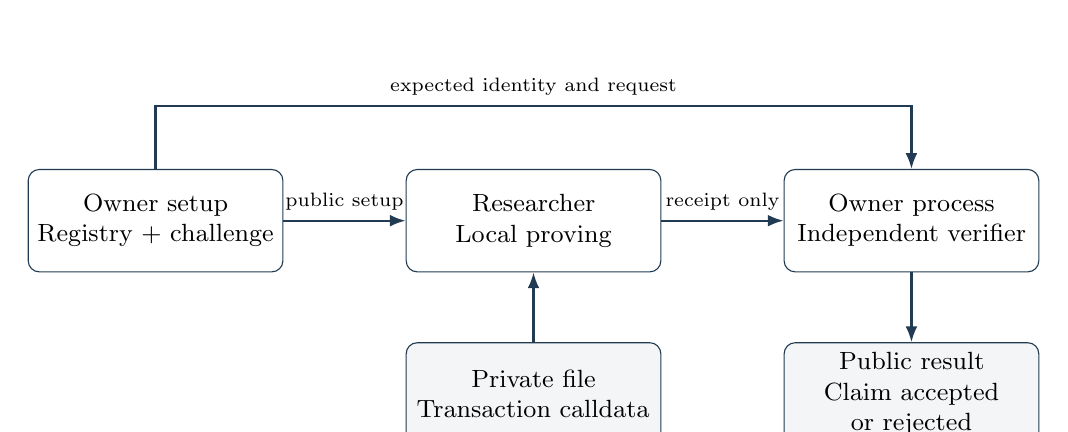
\begin{tikzpicture}[
  box/.style={draw=Ink,rounded corners,align=center,text width=3.0cm,
    minimum height=1.3cm,font=\small},
  flow/.style={-{Latex[length=2mm]},draw=Ink,thick}]
\node[box] (owner) at (0,0) {Owner setup\\Registry + challenge};
\node[box] (prover) at (4.8,0) {Researcher\\Local proving};
\node[box] (verifier) at (9.6,0) {Owner process\\Independent verifier};
\node[box,fill=Ink!5] (secret) at (4.8,-2.2) {Private file\\Transaction calldata};
\node[box,fill=Ink!5] (result) at (9.6,-2.2) {Public result\\Claim accepted or rejected};
\draw[flow] (owner) -- node[above,font=\scriptsize]{public setup} (prover);
\draw[flow] (prover) -- node[above,font=\scriptsize]{receipt only} (verifier);
\draw[flow] (secret) -- (prover);
\draw[flow] (verifier) -- (result);
\draw[flow] (owner.north) -- ++(0,0.8) -|
  node[above,pos=0.25,font=\scriptsize]{expected identity and request} (verifier.north);
\end{tikzpicture}
\caption{The secret terminates at the local prover. Verification uses independently trusted public setup.}
\end{figure}

The guest owns the statement's truth conditions. The host owns private input handling and computation scheduling, but cannot decide that the exploit succeeded. The verifier owns acceptance and cannot delegate that decision to a browser, receipt envelope, or prover-supplied image identifier.

\begin{longtable}{L{0.20\linewidth}L{0.35\linewidth}L{0.35\linewidth}}
\toprule
\textbf{Concern} & \textbf{Proposed canonical owner} & \textbf{Required boundary} \\
\midrule
\endhead
Vault semantics & \filepath{contracts/src/DemoVault.sol} and \filepath{contracts/src/PatchedVault.sol} & Same API and storage layout; explicit authorization repair. \\
Scenario encoding & \filepath{crates/model/src/scenario.rs} & One canonical byte encoding shared by guest and verifier. \\
Claim definition & \filepath{crates/model/src/claim.rs} & One predicate implementation; portal does not reproduce or score it. \\
EVM transitions & \filepath{crates/runner/src/lib.rs} & Consumes fixed state/environment and private calldata; returns structured post-state or failure. \\
Proved execution & \filepath{methods/guest/src/main.rs} & Recomputes digests, executes, asserts the predicate, then commits the exact journal. \\
Private proof generation & \filepath{crates/proof/src/prover.rs} & Local SDK prover; secret file never submitted to server or remote service. \\
Receipt acceptance & \filepath{crates/proof/src/verify.rs} & Strict receipt-type, image, journal, scenario, and challenge validation. \\
Request authority & \filepath{crates/cli/src/challenge.rs} & Creates nonce from OS randomness; owner supplies expected request separately. \\
Portal result & \filepath{crates/portal/src/main.rs} & Calls the same verifier library; serves public static interface over loopback. \\
\bottomrule
\end{longtable}

\section{Target and State Contracts}\label{sec:target}
\subsection{Contract Interface and Deliberate Defect}
Both vault variants use Solidity 0.8.26 with a single \code{mapping(address => uint256) public credit} at storage slot 0. They expose \code{deposit()} as payable and \code{withdraw(uint256 amount)} as nonpayable. There is no administrator, upgrade, recovery, token, or external registry function. A deposit requires a positive value and adds that value to the caller's credit using checked arithmetic.

The vulnerable withdrawal checks only that the amount is positive and the vault has sufficient native currency. It transfers that amount to \code{msg.sender} and requires transfer success. It omits the caller-credit authorization check and corresponding debit. This is a deliberately isolated accounting/authorization defect, not a reentrancy demonstration.

The patched withdrawal additionally requires \code{credit[msg.sender] >= amount}, subtracts the amount before the external transfer, and reverts on transfer failure. Reversion restores the ledger update. The API, mapping slot, deposit behavior, and fixture construction remain identical. No second defect is intentionally introduced. Unit tests must verify legitimate deposit/withdraw behavior for the patch as well as rejection of the reference unauthorized call.

In both variants, the native-currency transfer uses a low-level Solidity \code{call} to \code{payable(msg.sender)}, with \code{value: amount}, empty calldata, and the default forwarded gas. Require its Boolean success value. Do not substitute Solidity's \code{transfer} or \code{send}; those introduce different gas and failure behavior. No events or additional entry points are needed.

\begin{verbatim}
Vulnerable withdrawal:
  require(amount > 0)
  require(vault.balance >= amount)
  transfer amount to caller; require success

Patched withdrawal:
  require(amount > 0)
  require(vault.balance >= amount)
  require(credit[caller] >= amount)
  credit[caller] -= amount
  transfer amount to caller; require success
\end{verbatim}

These are design pseudocode, not files compiled during dossier preparation. The public code intentionally makes the defect understandable. The demo proves nondisclosure of a specific payload through the verification channel; it does not show that this obvious fixture bug remains unknown to someone who reads the code.

\subsection{Registered Accounts and Initial State}
Let \(T\) be the target, \(V\) the passive victim, and \(A\) the ordinary attacker. Addresses are fixed to the following 20-byte values, expressed as zero-padded hexadecimal integers: \(T=\mathtt{0x1001}\), \(V=\mathtt{0x2001}\), and \(A=\mathtt{0x3001}\). They must be nonzero and distinct. The latter two have no runtime code.

\begin{longtable}{L{0.17\linewidth}L{0.21\linewidth}L{0.25\linewidth}L{0.25\linewidth}}
\toprule
\textbf{Account} & \textbf{Native balance} & \textbf{Vault credit} & \textbf{Code and nonce} \\
\midrule
\endhead
Target \(T\) & \(10\cdot10^{18}\) wei & Not an owner of a credit & Compiled selected variant; nonce 1 \\
Victim \(V\) & 0 wei & \(10\cdot10^{18}\) wei & Empty code; nonce 1 after fixture deposit \\
Attacker \(A\) & 0 wei & 0 wei & Empty code; nonce 0 \\
\bottomrule
\end{longtable}

The fixture generator starts the victim with ten synthetic currency units and nonce 0, installs the public runtime at the synthetic target address with nonce 1, and executes the victim's ordinary deposit through \code{transact_call}. That setup call has origin \(V\), value \(10\cdot10^{18}\), and gas limit 500,000. Export its applied state, preserving the victim's resulting nonce 1. For proving, construct a fresh backend with the registered environment whose origin is \(A\). Runtime installation is an explicit genesis fixture facility; no on-chain deployment or inclusion is asserted. The target's only nonzero storage entry is the victim-credit slot. Both EOAs have empty storage and code. Initial state must match these constraints and the table exactly.

The victim-credit slot is \(\operatorname{Keccak256}(\operatorname{pad}_{32}(V)\|\operatorname{pad}_{32}(0))\). The analogous attacker slot must read zero. Compiler storage-layout output must confirm slot 0 rather than relying on an untested source-layout assumption. Zero-valued entries are omitted from the canonical storage vector; missing entries read as zero.

\subsection{Transaction and Environment}
The transaction's caller is \(A\), destination is \(T\), value is zero, access list is empty, and gas limit is 500,000. Only calldata is private. The sender is never selected from input. The private data limit is 256 bytes. A reference payload ABI-encodes a withdrawal of \(10^{18}\) wei; no witness is placed on the command line.

The interpreter selects \code{Config::cancun()}. The environment fixes origin \(A\), chain ID 31337, block number 1, timestamp 1, coinbase zero, difficulty zero, base fee zero, gas price zero, block gas limit 500,000, and an empty historical block-hash list. The pinned \code{MemoryVicinity} also requires \code{block_randomness}; set it to \code{Some(H256::zero())}, never \code{None}, and commit its presence and bytes \cite{evmsource}. Undefined historical hashes read zero under this synthetic model. These fields exhaust the pinned vicinity structure; future fields require an explicit model revision. The host must not fetch live values or inherit mutable RPC settings.

Gas is a resource bound, not a monetary expense in this fixture. A proof therefore demonstrates value extraction under a zero-fee sandbox and does not establish economic profitability on a network. The target has no precompile interactions or dependence on block context. The selected runner is not claimed to be a complete Ethereum client. Any discovered unsupported operation on a reachable path blocks promotion until the model is corrected or the target is further restricted.

\subsection{EVM Adapter and Post-State}
Use \code{MemoryBackend}, \code{StackSubstateMetadata::new(500000, ...)}, \code{MemoryStackState}, and \code{StackExecutor::new_with_precompiles} with an empty precompile map. Execute exactly one \code{transact_call(A, T, 0, calldata, 500000, empty_access_list)}. This entry point charges intrinsic calldata gas and increments the caller's nonce; a lower-level message call must not replace it \cite{evmsource}. No signature, fee settlement, transaction-pool validation, or full block processing is modeled.

On \code{ExitReason::Succeed}, consume \code{executor.into_state()}, obtain its \code{deconstruct()} changes and logs, and apply them once through \code{ApplyBackend::apply(..., delete_empty=true)}. Inspect the resulting backend, not an unchanged clone or a hand-adjusted balance table. Omit zero slots during canonical extraction, preserve untouched accounts, and check that the accepted transaction leaves nonces \(N_A=1\), \(N_V=N_T=1\). Fresh backends prevent retained warm-access or transient-storage state. Revert, error, fatal exit, or exhaustion never produces the successful claim journal. Diagnostics may inspect a rejected transition privately, but its transaction-level nonce change must not be confused with successful contract effects.

The native adapter and guest call the same transition function. Foundry comparison uses the exact compiled runtime installed at \(T\), the fixed ledger and balances, the same sender/value/calldata, and the same hardfork. Foundry's message-call harness does not reproduce the transaction envelope; compare success/revert, balances, credits, and code identity there. Check transaction nonce and intrinsic-gas behavior separately in adapter tests. Contract-level gas exhaustion is tested in both paths without requiring identical harness gas totals.

\section{Formal Statement and Impact Predicate}
\subsection{Quantities and Arithmetic}
Balances and credits are unsigned 256-bit integers measured in synthetic wei. Their values are not fiat amounts, severity classes, or probabilities. Nonces and gas limits are counters. Digests and challenge nonces are byte strings, with no arithmetic interpretation. The dossier is not physics-facing; dimensional analysis of physical models is inapplicable. Integer bounds, conservation, and subtraction order are the relevant consistency checks here.

Let \(S_0\) be the registered pre-state and \(S_1\) the state after executing calldata \(w\). Denote account balances by \(B_X(S)\), vault ledger credits by \(C_X(S)\), and account nonces by \(N_X(S)\). Define differences only after checking their ordering:
\begin{align}
\Delta_A &= B_A(S_1)-B_A(S_0), && B_A(S_1)>B_A(S_0),\\
L_T &= B_T(S_0)-B_T(S_1), && B_T(S_0)>B_T(S_1).
\end{align}
No modular underflow, saturating subtraction, floating-point conversion, or signed cast may convert a failed ordering into a positive impact. Checked arithmetic is required for sums.

The fixed unauthorized-withdrawal predicate is
\begin{equation}
\begin{aligned}
P(S_0,S_1) ={}& \operatorname{TransactionSucceeded}\ \land\ C_A(S_0)=0\ \land\ C_A(S_1)=0\\
&\land\ C_V(S_1)=C_V(S_0)=10\cdot10^{18}\\
&\land\ B_V(S_1)=B_V(S_0)=0\\
&\land\ \Delta_A=L_T\geq 1\text{ wei}\\
&\land\ B_T(S_1)<C_V(S_1)\\
&\land\ \operatorname{TargetCodeUnchanged}\ \land\ \operatorname{EOACodeEmpty}\\
&\land\ N_A(S_1)=1\ \land\ N_V(S_1)=N_T(S_1)=1.
\end{aligned}
\end{equation}
The scenario also requires total post-state native balance across \(T,V,A\) to equal \(10\cdot10^{18}\) wei and no new accounts with nonzero balance or code. This captures the declared closed-world fixture and catches accidental state application or balance-override errors. The minimal one-wei threshold detects a positive unauthorized transfer. It is not a severity threshold.

Because the victim is the only depositor, the attacker has no credit, the victim's credit remains owed, and the vault loses exactly the attacker's gain, the predicate attributes the deficit to extraction of funds backing the victim's deposit. This reasoning depends on the fixed fixture; it must not be generalized to an arbitrary contract or accounting model.

\subsection{Proof Relation}
Let \(E\) be the registered environment, \(d\) the scenario digest, \(n\) the owner's challenge nonce, and \(I\) the trusted guest image ID. The guest proves knowledge of \(w\) such that
\begin{equation}
\begin{aligned}
& |w|\leq256,\qquad d=\operatorname{ScenarioDigest}(S_0,E,T,V,A),\\
& S_1=\operatorname{Execute}_{\mathrm{Cancun}}(S_0,E,A,T,0,w,500000),\\
& P(S_0,S_1)=\mathrm{true},\\
& J=\operatorname{EncodeJournal}(d,n,1).
\end{aligned}
\end{equation}
The SDK receipt binds a successful guest execution with image \(I\) to journal \(J\). The guest recomputes every scenario commitment from its execution inputs. Merely accepting a digest asserted by the host is insufficient. The verifier compares the resulting digest with its separately registered expectation.

\subsection{Limits of the Assertion}
Acceptance establishes the existence of an input satisfying this bounded relation, under the SDK and interpreter assumptions. It does not establish authorship, discovery priority, deployed-chain applicability, maximum loss, severity, or correctness of all code. A failed witness, out-of-gas result, rejected proof, or lack of a proof does not establish safety. The patched demonstration means \emph{the same reference payload no longer satisfies the predicate}; it does not prove universal absence of vulnerabilities.

\section{Data and Artifact Contracts}
\subsection{Canonical Encodings}
JSON is a readable transport for setup, not the hashed representation. All canonical encodings are implemented once in the model crate and tested with independent byte-vector fixtures. Integer encodings below are explicit; locale, whitespace, object ordering, and decimal formatting must not affect the committed bytes. Lengths and counts are unsigned little-endian integers. Monetary and storage words are exactly 32 bytes, unsigned big-endian.

\begin{longtable}{L{0.21\linewidth}L{0.43\linewidth}L{0.26\linewidth}}
\toprule
\textbf{Object} & \textbf{Canonical layout} & \textbf{Validation} \\
\midrule
\endhead
State & Eight-byte magic \code{PSPHS001}; u32 account count; sorted account records. Each record: address[20], nonce u64, balance[32], code length u32 and code, storage count u32, sorted key[32]/value[32] pairs. & At most 32,768 bytes; exactly \(T,V,A\). Target runtime is 1--24,576 bytes; only its victim slot is nonzero. EOAs have no code or storage. \\
Environment & Magic \code{PSPHE001}; Cancun tag u8=1; chain ID[32], origin[20], gas price[32], block number[32], coinbase[20], timestamp[32], difficulty[32], block gas limit[32], base fee[32]; randomness-present u8=1 and randomness[32]=0; historical hash count u32=0. & Exactly 310 bytes. Every field equals the fixed environment in Section~\ref{sec:target}; no unspecified defaults. \\
Claim descriptor & ASCII \code{ProofSphere/unauthorized-withdrawal/v1}, then maximum calldata u16=256, transaction gas u64=500,000, minimum gain[32]=1 wei. & Encodes constants; actual predicate is governed by the independently pinned guest. \\
Scenario descriptor & Magic \code{PSPHSC01}; \(T,V,A\) addresses[20] each; code digest[32], state digest[32], environment digest[32], claim digest[32]. & Exactly 196 bytes. Digests recomputed inside guest. \\
Journal & Magic \code{PSPHJ001}; scenario digest[32]; challenge nonce[32]; claim flag u8=1. & Exactly 73 bytes, with no suffix or optional fields. \\
\bottomrule
\end{longtable}

All four constituent digests and the scenario digest use SHA-256. The code digest hashes the selected target's deployed runtime bytes directly. The state, environment, and claim digests hash their canonical encodings. The scenario digest hashes the 196-byte descriptor. Ethereum's Keccak-256 remains the required operation for mapping-slot derivation; it is not interchangeable with SHA-256. The image ID uses the SDK's own computation and serialization, not a custom conversion of its internal words.

Nonce values in setup must fit u64; the fixed fixture uses only 0 and 1. Invalid widths, duplicate JSON keys, duplicate accounts, duplicate storage keys, unknown fields, unsupported version markers, truncated data, and trailing bytes are rejected. Canonical vectors must already be ordered; decoders must not quietly deduplicate malformed submissions. JSON balances are decimal strings parsed as bounded unsigned integers, never JavaScript numbers.

\subsection{Public Setup Schemas}
Each fixture directory contains \code{state.json} and \code{environment.json}. All fields below are required; no extra fields are accepted. Each JSON file is bounded to 64 KiB before parsing. Unsigned JSON integers, including nonces and environment counters, are decimal strings without signs or leading zeroes, except \code{"0"}. Addresses are \code{0x} plus 40 lowercase hexadecimal digits; code is \code{0x} plus an even number of lowercase digits, including \code{0x} for empty code. Storage keys/values are \code{0x} plus 64 digits. SHA-256 digests and challenge nonces are 64 lowercase hex digits without \code{0x}. Guest image IDs use the SDK's \code{Digest} display/parse representation, with a tested round trip rather than manual word conversion.
\begin{longtable}{L{0.24\linewidth}L{0.66\linewidth}}
\toprule
\textbf{Object} & \textbf{Exact JSON field set} \\
\midrule
\endhead
State & \code{format = proofsphere-state-v1}, \code{accounts}. Each account: \code{address}, \code{nonce}, \code{balance}, \code{code}, \code{storage}. Each storage entry: \code{key}, \code{value}. Account and storage arrays are already sorted by decoded bytes. \\
Environment & \code{format = proofsphere-environment-v1}, \code{hardfork = cancun}, \code{chain_id}, \code{origin}, \code{gas_price}, \code{block_number}, \code{coinbase}, \code{timestamp}, \code{difficulty}, \code{gas_limit}, \code{base_fee}, \code{block_randomness}, \code{block_hashes}. Randomness is the fixed 32-byte zero hex string; hashes are an empty array. \\
Registry & \code{format = proofsphere-registry-v1}, \code{scenarios}. Each entry: \code{id}, \code{label}, \code{state_file}, \code{environment_file}, \code{code_digest}, \code{state_digest}, \code{environment_digest}, \code{claim_digest}, \code{scenario_digest}, \code{guest_image_id}. Sort entries by ID; paths are relative to the registry directory. \\
Challenge & \code{format = proofsphere-challenge-v1}, \code{scenario_id}, \code{scenario_digest}, \code{guest_image_id}, \code{nonce}. All identities must match the separately selected trusted entry. \\
\bottomrule
\end{longtable}
Only the state account record owns executable runtime bytes; a registry digest is derived data, not a second code source. The shared model owns the fixed addresses and claim constants. Compiler tooling emits runtime and storage-layout evidence; fixture generation verifies that the target account contains that runtime. Registry loading recomputes every digest from the referenced public files and fails on inconsistency. Generated fixture paths must stay under the fixtures directory.

\subsection{Bounded Guest Input}
The host sends raw bytes through \code{ExecutorEnv} slice input. The guest reads stdin through bounded fixed-buffer reads rather than unbounded \code{Vec} deserialization. The layout is magic \code{PSPHI001}, state length u32 and canonical state bytes, environment length u32 and canonical environment bytes, nonce[32], calldata length u16 and calldata bytes. Enforce the 32,768-byte state cap, exact 310-byte environment length, 256-byte calldata cap, and end of input. Read and validate each length before allocating its field. The guest derives the code and claim digests itself; no host-supplied success or claimed digest is needed. The model's decoders own both structural bounds and semantic validation.

\subsection{Owner Registry and Challenge}
\filepath{fixtures/registry.json} contains two named entries: \code{vault-vulnerable-v1} and \code{vault-patched-v1}. Each entry identifies its public setup files, generated constituent digests, scenario digest, and the expected guest image ID. Both variants use the same generic guest; their different runtime bytecode yields different code and state digests. The registry is generated from a trusted build and is immutable to proof submissions. No registration HTTP endpoint exists in v1.

A challenge uses the exact schema above and a uniformly random 32-byte nonce obtained from OS randomness. The verifier takes its image ID from the trusted registry/build, compares the challenge's convenience copy, and takes the expected nonce from the separately supplied owner challenge. A challenge bundled by a claimant is insufficient authority. The CLI must refuse an ID, digest, or image mismatch before proving or verifying.

The CLI permits repeat verification of the same owner request. The portal keeps one active challenge in memory. Issuing a new challenge or switching scenarios invalidates the previous active request. Restarting loses the active request unless the owner explicitly loads a recorded challenge at startup. There is no timestamp freshness proof, payment, or durable anti-replay ledger. A receipt for a different nonce is rejected; reverification under the same nonce is idempotent. Recorded mode is selected by \code{--recorded-challenge <path>} when launching the portal. Validate that owner-supplied file against the trusted registry before serving it. There is no browser challenge-import endpoint. Creating a fresh challenge exits recorded mode.

\subsection{Private Witness}
The witness is a binary file containing at most 256 calldata bytes. It has no sender, destination, value, code, state, environment, or claim fields. The prover opens it locally, supplies its bytes to the guest, and releases only the receipt. A proposed \code{demo-witness} command creates the reference ABI payload in \filepath{.proofsphere-private/reference.bin} with restrictive user-only permissions. This directory, temporary traces, and private inputs are ignored by Git. Tests can derive the known reference input without committing the generated witness file.

The host must not derive \code{Debug} output for witness-containing types or print payloads, call selectors, decoded arguments, execution traces, memory dumps, or returndata. The portal has no witness picker, secret-upload endpoint, or prover service. SDK proof assets may be obtained before rehearsal, but proof generation itself must not transmit private inputs. Remote/Bonsai proving is disabled for this version.

\subsection{Proof Container}
A \code{.psproof} file consists of magic \code{PSPHP001} (8 bytes), receipt payload length (u64 little-endian), and the exact receipt payload. Payload length must not exceed 8 MiB; the complete file cannot exceed 8 MiB plus 16 bytes. The pinned SDK \code{Receipt} is encoded with bincode 1.3.3 using fixed-integer, little-endian options, a size limit, and rejection of trailing bytes. All writers and readers use the same options; SDK upgrades require a new container version and regenerated artifacts.

The external envelope contains no asserted image ID, success field, exploit description, or raw witness. The public claim comes only from the verified journal. The verifier first bounds the file and lengths, then bounds deserialization. It accepts only \code{InnerReceipt::Succinct}. Fake, composite, Groth16, and unknown variants are rejected in v1. Other authentic receipt types may be added only with an explicit privacy/format review and a versioned decision; fake receipts can never become accepted evidence.

\section{Proving and Verification Algorithms}
\subsection{Guest Procedure}
\begin{enumerate}
\item Read the bounded raw input described above: public setup bytes, nonce[32], and private calldata. Validate lengths before allocating fields.
\item Decode and validate addresses, sorted account records, exact initial balances/credits, EOA code/storage, code size, nonces, environment, and calldata length. Derive the code digest from the target runtime.
\item Compute the canonical state, environment, claim, and scenario digests. These values describe the exact data subsequently executed. Do not maintain an independently mutable hashed copy and execution copy.
\item Construct the EVM memory backend from that same validated state. Execute one call with fixed \(A,T\), zero value, empty access list, and gas limit 500,000.
\item Deconstruct and apply the executor's final state through the specified adapter. Reject revert, error, fatal exit, exhaustion, unsupported reachable behavior, or malformed result.
\item Check the complete impact predicate and conservation conditions using checked integer arithmetic. A failed predicate terminates without a successful claim journal.
\item Commit the 73 journal bytes containing the computed scenario digest, supplied nonce, and true flag. No private diagnostics or final balances are committed.
\end{enumerate}

The guest does not verify external assumptions or take host assertions of success. Its only authority is its executed code. Input data may be private to the proof system even when semantically public; correctness comes from digest recomputation and verifier comparison.

\subsection{Local Host Procedure}
Load the selected registry setup and challenge, validate them, and read the bounded witness file. For the host, pin \code{risc0-zkvm = "=3.0.6"} with \code{default-features=false} and explicit \code{prove} and \code{disable-dev-mode} features. Instantiate \code{LocalProver::new("proofsphere-local")} directly; do not call \code{default_prover()}, which can select another backend from the environment. Use \code{ProverOpts::succinct().with_dev_mode(false)} with \code{prove_with_opts} and an explicitly production verifier context \cite{risc0prover,risc0local}. Startup rejects a nonzero \code{RISC0_DEV_MODE}, any \code{BONSAI_API_URL} or \code{BONSAI_API_KEY}, and a nonempty \code{RISC0_PROVER} other than \code{local}. The build must not enable \code{bonsai}; inspect the resolved feature tree, not only one manifest.

Initial local execution settings are \code{segment_limit_po2(20)} and \code{session_limit(Some(1 << 27))}. They bound segment memory and total guest cycles through the pinned executor API \cite{risc0env}; the 500,000 EVM gas bound is a separate quantity. These are operational limits, not severity or public claim fields. Measure them in the proof gate and record any justified revision before promotion. A cycle-limit failure produces no accepted artifact. Run real proving and compression in a release build; a development receipt or debug-build timing is not demonstration evidence.

After generation, require a succinct inner receipt and locally verify it with the expected image and context. Parse and compare the complete journal against the intended setup and challenge. Only then write a temporary file in the destination directory and atomically persist it without replacing an existing path. Refuse existing outputs so a failed retry cannot leave an old receipt looking fresh. On failure, remove the temporary file and write no success artifact or green result. Private performance measurements and intermediates remain under \filepath{.proofsphere-private/}; they never accompany the receipt.

\subsection{Independent Verifier Procedure}
\begin{verbatim}
verify(file, trusted_registry_entry, owner_challenge):
  bound and decode the container; reject trailing bytes
  require receipt type == Succinct
  use production verifier context; dev mode == false
  verify receipt against registry's expected guest image ID
  require journal length == 73 and magic == PSPHJ001
  require journal.scenario == registry.scenario
  require challenge.scenario == registry.scenario
  require journal.nonce == challenge.nonce
  require journal.claim_flag == 1
  return Accepted(UnauthorizedWithdrawalDemonstrated)
\end{verbatim}

The release verifier enables the pinned SDK's \code{disable-dev-mode} feature and explicitly uses \code{VerifierContext::default().with_dev_mode(false)} with \code{verify_with_context}. It also checks the receipt enum directly; environment defaults are never sufficient. It must reject fake receipts when launched from a shell with \code{RISC0_DEV_MODE=1}, while continuing to accept a genuine matching succinct receipt. SDK source shows that default context behavior can depend on environment; this motivates the explicit controls \cite{risc0receipt}.

The proof crate's optional \code{prove} feature owns local proving and the generated guest ELF dependency; its default is verifier-only. The CLI enables proving for its researcher build. The portal depends on the verifier-only build and public registry, so it requires neither private files nor proving assets. Each independently distributed binary records its exact SDK/feature configuration. Use the SDK's default production verifier parameters; never load them from an artifact.

\subsection{Failure Semantics}
\begin{longtable}{L{0.31\linewidth}L{0.59\linewidth}}
\toprule
\textbf{Result code} & \textbf{Meaning and user-facing behavior} \\
\midrule
\endhead
\code{UNSUPPORTED_FORMAT} & Bad magic, version, receipt type, or exact-length constraint. Show ``Unsupported proof artifact.'' \\
\code{TOO_LARGE} & Body or bounded payload exceeds the cap. Reject before expensive work. \\
\code{RECEIPT_REJECTED} & Cryptographic verification or expected image check failed. Show ``Proof could not be verified.'' \\
\code{SCENARIO_MISMATCH} & Verified journal does not refer to the independently selected scenario. \\
\code{CHALLENGE_MISMATCH} & Receipt belongs to a different owner request. \\
\code{CLAIM_INVALID} & Journal has an invalid flag, layout, or extra bytes despite a valid receipt. \\
\code{NO_ACTIVE_CHALLENGE} & Portal requires a current owner request before accepting an upload. \\
\code{REQUEST_REPLACED} & Active scenario/request changed while an upload or verification was pending; discard its result. \\
\code{BUSY} & One verification is already admitted. Retry after it completes; no second job is queued. \\
\code{GENERATION_FAILED} & Local execution or proof generation failed. This is not evidence that the contract is safe. \\
\bottomrule
\end{longtable}

The CLI returns exit code 0 only for accepted verification, 2 for a rejected claim/artifact, and 3 for an operational error such as an unreadable trusted registry. JSON results use \code{status = accepted|rejected|error}; only accepted results contain \code{claim = unauthorized-withdrawal-demonstrated}. Rejection messages omit private execution state. The browser treats operational failure separately from rejection and never restores a stale accepted badge.

\section{Portal and Demonstration Experience}
\subsection{Interaction Model}
The portal is a static HTML/CSS/JavaScript application served by a Rust verifier process bound to \code{127.0.0.1:4173}. It has one main workflow and no accounts or role-management system. Selecting a scenario creates a fresh owner challenge through the server; the owner can replace it explicitly, download its public file, and verify an uploaded proof. A configured recorded challenge is shown as the initial selection without silently replacing its nonce. A separate researcher instruction panel shows a CLI invocation with file paths, not a payload. It clearly states that the witness stays on the researcher's machine.

Before any upload, the browser reads only the first 16 bytes locally and validates the proof magic, declared length, and file cap. A mistaken witness selection is rejected before a request is sent. The server repeats all validation. The browser is not a cryptographic verifier and cannot set an accepted result itself; the independent CLI remains an additional verification path.

\begin{longtable}{L{0.24\linewidth}L{0.35\linewidth}L{0.31\linewidth}}
\toprule
\textbf{Surface} & \textbf{Behavior} & \textbf{Invariant} \\
\midrule
\endhead
Scenario summary & Show variant, synthetic vault, fixed caller, and claim explanation. Expandable detail shows public hashes. & Labels come from the trusted registry. \\
Request & Create or select a recorded owner challenge; show a shortened request identifier. & Switching requests clears file selection and prior result. \\
Proof selection & Choose only bounded \code{.psproof} files; local magic check precedes upload. & No secret input picker or uploaded exploit source. \\
Verification & Idle, selected, verifying, accepted, rejected, or operational error. Disable duplicate submission. & No green result before a successful server response. \\
Accepted report & ``Unauthorized withdrawal demonstrated'' plus target/request identities. & No severity, maximum loss, safety badge, or authored-by claim. \\
Rejected report & Explain mismatch or unsupported artifact in plain language. & No implication that the target is secure. \\
Recorded mode & Persistent label: ``Recorded proof; verification performed now.'' & No simulated generation spinner or fresh-challenge claim. \\
\bottomrule
\end{longtable}

Visual requirements include keyboard-operable inputs, visible focus, labeled file controls, a text explanation beside status color, a live status region, and no horizontal overflow at widths 390 and 1280 pixels. Raw technical hashes belong in expandable provenance details. The primary flow explains the security outcome in ordinary language. On target/request change, clear acceptance immediately and disable upload until the server confirms the new request. Apply an async response only when its captured scenario, nonce, and generation match the current selection; otherwise discard it. Disable challenge controls while their mutation request is pending, so older challenge responses cannot overwrite a newer selection.

\subsection{HTTP Contract}
\code{GET /api/scenarios} returns \code{scenarios} and \code{active_request}; the latter is null or contains \code{scenario_id}, \code{nonce}, \code{generation}, and \code{mode = fresh|recorded}. Generation is a process-local u64 counter represented as a decimal string. It is never part of the cryptographic journal or challenge file.

\code{POST /api/challenge} accepts a JSON object whose sole field is \code{scenario_id}, with a registered ID and a 1 KiB body limit. It replaces the active request with a fresh OS-generated nonce, increments generation, and returns \code{challenge}, \code{generation}, and \code{mode = fresh}. \code{GET /api/challenge} downloads the exact active challenge schema, or reports \code{NO_ACTIVE_CHALLENGE}.

\code{POST /api/verify} accepts \code{application/octet-stream}, the proof-file cap, and \code{X-ProofSphere-Generation} equal to the browser's captured generation. Before decoding, acquire the single-job permit and snapshot the active trusted registry entry, nonce, mode, and generation. Perform the shared-library verification outside the async executor. Before returning acceptance, compare that snapshot with the current request. A replacement produces \code{REQUEST_REPLACED} without an accepted claim. Hold the permit until the worker actually finishes; browser cancellation must not admit overlapping work.

Verification JSON contains \code{status}, \code{code}, \code{scenario_id}, \code{nonce}, \code{generation}, and \code{mode}; only acceptance includes \code{claim} and \code{verification_ms}. Context fields identify the server's expected request, not an assertion extracted from an unverified file. Use HTTP 200 for completed accepted/rejected verification, 400 for malformed request, 413 for size rejection, 409 for absent/replaced request or busy admission, and 500 for operational failure. Every error response has structured status/code; HTTP 200 alone never means acceptance.

Mutations require \code{X-ProofSphere-UI: 1}. Validate the exact loopback Host and, when present, the matching Origin; emit no permissive CORS headers. The service performs no shell execution, witness reading, remote proving, RPC call, or target registration from HTTP input. Proving and independent verification use the CLI. No hosted deployment is required.

\section{Stack Selection and Alternatives}
\begin{longtable}{L{0.24\linewidth}L{0.29\linewidth}L{0.37\linewidth}}
\toprule
\textbf{Component} & \textbf{Baseline} & \textbf{Reason and readiness} \\
\midrule
\endhead
Guest SDK/build & \code{risc0-zkvm = "=3.0.6"}, \code{risc0-build = "=3.0.6"} & Defaults disabled. Guest uses \code{std}; local host uses \code{prove, disable-dev-mode}; verifier uses \code{std, disable-dev-mode}. Integration untested. \\
Host Rust & 1.97.0 explicit toolchain & Matches inspected release repository toolchain; installed locally but not the active default. \\
Guest tooling & \code{r0vm} and \code{cargo-risczero} 3.0.6; RISC Zero Rust 1.97.0 & Pin all components; guest Rust release \code{r0.1.97.0} is published. Tools were not found locally. \\
EVM & \code{evm = "=0.42.0"}, Cancun & Used by the inspected reference; avoids adopting a different interpreter and changing scope concurrently. \\
Solidity & \code{solc = 0.8.26} via standard JSON & Explicit Cancun; optimizer enabled, 200 runs; metadata bytecode hash set to none. Verify full compiler version and output errors. \\
Container & bincode 1.3.3 with explicit options & Stable bounded receipt serialization; SDK version is part of compatibility authority. \\
Compiler tools & Node 22.23.1, pnpm 11.25.0 & Local versions inspected; package manager and solc dependency are pinned in the proposed compiler-tools manifest. \\
Portal & Plain HTML/CSS/JS; Rust Axum 0.8 API family & Small presentation layer. Resolve exact Axum/Tokio and support versions once, retain Cargo.lock, then use locked builds. \\
Independent contract tests & Foundry plus native runner tests & Record exact tested Foundry release before promotion; no installed Foundry was observed. \\
\bottomrule
\end{longtable}

Support dependencies are not claimed to have resolved locks. Phase 0 records the workspace and guest locks; Phase 1 records the compiler-tool lock and exact tested Foundry version. Retain all of them with the toolchain manifest before the first exploit proof is promoted. The proof gate must demonstrate that the selected SDK/interpreter combination builds and genuinely proves. If it fails, record the actual error and revise the baseline before building the portal. An older SDK or mock receipt is not an implicit fallback.

\begin{longtable}{L{0.24\linewidth}L{0.18\linewidth}L{0.48\linewidth}}
\toprule
\textbf{Alternative} & \textbf{Disposition} & \textbf{Tradeoff} \\
\midrule
\endhead
Whole existing zkpoex application & Reference only & Its host/environment, logging, public claim, and development defaults need adaptation; its chain and payment paths exceed the selected scope. \\
Custom Noir arithmetic circuit & Defer & Smaller computation, but a rewritten vault model does not prove execution of Solidity runtime bytes. Avoid that semantic substitution. \\
Private attacker bytecode inside an EVM & Defer & Supports richer exploits but adds code installation, deployment assumptions, and witness complexity. Direct calldata suffices for this fixture. \\
Live chain/fork & Defer & Requires authenticated state and independently checked canonical block identity; not necessary for the first product test. \\
Hosted proof generation & Exclude & The operator receives the private witness unless an additional confidentiality mechanism is designed. \\
Severity disclosure & Defer & Needs policy, thresholds, and careful lower-bound interpretation; it does not improve the first Boolean proof demonstration. \\
Groth16/on-chain verification & Defer & Payment or on-chain use is absent; local succinct verification avoids an additional prover/deployment layer. \\
Signed JSON assertion or animation & Reject & Does not establish the computation through the proof system. \\
\bottomrule
\end{longtable}

\section{Implementation Plan and File Map}
\subsection{Gated Sequence}
\begin{enumerate}
\item \textbf{Phase 0: proof tooling.} Create the minimal Rust workspace/guest skeleton and a real-receipt integration test. Pin SDK features and tools, generate Rust locks, and prove a minimal guest in release mode with genuine succinct receipts and development mode disabled. Verify separately; confirm fake rejection. Exit only on a genuine accepted receipt. This establishes tooling, not EVM compatibility or the exploit claim.
\item \textbf{Phase 1: target and ordinary behavior.} Write failing tests for the patched authorization requirement and legitimate deposit/refund; the vulnerable characterization test deliberately expects the uncredited gain. Implement both variants. Compile with fixed settings, record the compiler lock and Foundry version, check storage layout, and construct both snapshots. Exit when the vulnerable reference call gains funds, the patch rejects it, and legitimate patched withdrawals work.
\item \textbf{Phase 2: first real vault proof.} Write relation, canonical encoding, substitution, state-application, and arithmetic tests. Implement runner/model and guest checks; compare contract behavior with Foundry. Build the final guest, then generate the registry from its image ID and fixtures. Produce a genuine succinct vault receipt and verify its exact journal in a separate minimal process. Retain it privately until the public format/output checks pass. Exit on the actual exploit claim; a minimal non-EVM receipt is insufficient.
\item \textbf{Phase 3: private proof artifact.} Add a real exploit-receipt test and strict verifier tests before wiring the CLI. Implement witness-file handling, local proving, bounded serialization, independent verification, and coarse logging. Exit when a separate verifier accepts a real exploit proof without its witness and rejects all required negative cases.
\item \textbf{Phase 4: portal and rehearsal.} Test request switching, malformed file selection, pending status, and stale responses. Build the loopback portal over the existing verifier library. Validate visually and rehearse genuine recorded or live proving mode. No portal-only acceptance path is permitted.
\item \textbf{Phase 5: evidence and completion.} Run focused tests and applicable full project checks, perform owner-clean after meaningful code changes, capture the artifact/privacy/rehearsal evidence, and regenerate this dossier if decisions changed. Stop when the exit rule is satisfied.
\end{enumerate}

The first useful implementation milestone is the end of Phase 3: the local CLI generates a real vault artifact, an owner process verifies it using public assets only, and the same reference payload fails on the patch. The portal makes that established result presentable. It does not resolve proof feasibility and must follow the milestone. Keep the selected module boundaries, but do not build a general plugin system, task scheduler, or configurable claim language.

\subsection{Proposed Repository Layout}
Every path below is proposed. The current creation pass writes the dossier and companion PDF only.
\begin{longtable}{L{0.39\linewidth}L{0.51\linewidth}}
\toprule
\textbf{Path or group} & \textbf{Implementation responsibility} \\
\midrule
\endhead
\filepath{Cargo.toml}, \filepath{Cargo.lock}, \filepath{rust-toolchain.toml} & Workspace membership, dependency pins, release profile, explicit host toolchain. \\
\filepath{contracts/src/DemoVault.sol}, \filepath{contracts/src/PatchedVault.sol} & Intentionally broken and repaired accounting behavior. \\
\filepath{contracts/test/Vault.t.sol}, \filepath{contracts/foundry.toml} & Independent behavior tests; matching compiler and Cancun settings. \\
\filepath{tools/contracts/package.json}, \filepath{tools/contracts/compile.mjs} & Locked solc standard-JSON compilation; runtime and storage-layout output; errors parsed from JSON. \\
\filepath{crates/model/src/scenario.rs}, \filepath{claim.rs}, \filepath{journal.rs}, \filepath{input.rs} & Public JSON, canonical setup, predicate, journal and bounded guest input; latter files share the model directory. \\
\filepath{crates/runner/src/lib.rs}, \filepath{tests/runner.rs} & EVM adapter, state application, bounded execution; tests under the runner crate. \\
\filepath{methods/build.rs}, \filepath{methods/guest/src/main.rs}, \filepath{methods/guest/Cargo.lock} & Compiled guest/image generation and guest dependency lock. \\
\filepath{crates/proof/src/prover.rs}, \filepath{verify.rs}, \filepath{container.rs}, \filepath{Cargo.toml} & Optional proving feature, verifier-only default, strict acceptance and bounded receipt format; source files share proof/src. \\
\filepath{crates/proof/tests/real_receipt.rs}, \filepath{verifier_adversarial.rs} & Expensive genuine receipts and rejection tests; latter test resides in the same tests directory. \\
\filepath{crates/cli/src/main.rs}, \filepath{challenge.rs}, \filepath{fixture.rs} & Package \code{proofsphere-cli}, binary \code{proofsphere}; fixture, registry, challenge, demo witness, prove, and verify commands. Other modules share cli/src. \\
\filepath{crates/portal/src/main.rs}, \filepath{apps/portal/index.html}, \filepath{app.js}, \filepath{styles.css} & Separate verifier-only binary \code{proofsphere-portal}; loopback service and static UI. JS/CSS reside in apps/portal. \\
\filepath{fixtures/registry.json}, \filepath{fixtures/vault-vulnerable/}, \filepath{fixtures/vault-patched/} & Each fixture directory holds state.json/environment.json; registry derives digests and trusted final guest identity. \\
\filepath{evidence/demo/}, \filepath{.proofsphere-private/} & Public accepted receipts/verifier reports; ignored witnesses, proving performance, and intermediates. \\
\filepath{README.md}, \filepath{.gitignore} & Reproduction instructions, explicit claim limits, and private/generated file exclusions. \\
\bottomrule
\end{longtable}

\subsection{Compatibility and Change Control}
No legacy format exists. Version 1 admits only its exact scenario, journal, and container formats. A semantic predicate change bumps the claim version and rebuilds the guest, registry, and receipts. An SDK/receipt-codec change bumps container format and proof assets. A contract change regenerates its runtime, snapshot, and scenario digest. The old receipt remains evidence for its old registered scenario; it cannot become evidence for the patched code. No silent aliases, inferred version fallback, or client-supplied trust roots are retained.

The v0.2 review changes an unimplemented baseline; no v1 proof assets already exist. Build order is contracts and compiler outputs, then fixture snapshots, then the guest, then its registry and receipts. The guest never embeds the registry or its own image ID. That avoids a build cycle and lets both variants use one image. Rebuilding the final guest after Phase 0 invalidates that phase's image identity for the exploit claim.

\section{Test-Driven Development Contract}
Tests must establish the behavior independently of an attractive interface. Contract tests deliberately distinguish the vulnerable fixture from the patched security requirement; the intentional vulnerability is not repaired in both variants. Development-mode execution may help diagnose the guest, but does not count toward genuine-receipt acceptance.

\begin{longtable}{L{0.25\linewidth}L{0.31\linewidth}L{0.34\linewidth}}
\toprule
\textbf{Test family} & \textbf{Failure established first} & \textbf{Required accepted result} \\
\midrule
\endhead
Contract authorization & An uncredited account can withdraw on the deliberately broken code. & Vulnerable test confirms the gain; patched security test rejects it. \\
Legitimate behavior & Incorrect patch can prohibit all withdrawals. & A funded depositor receives only its credited amount; debit is correct; repeated over-withdrawal fails. \\
Impact boundary & Zero gain, reverted calls, or unsigned subtraction can be misclassified. & One-wei unauthorized gain passes; zero gain, zero amount, over-balance request, revert, and exhaustion fail. \\
Encoding authority & Whitespace or malformed duplicate records can alter identity handling. & Independent golden bytes agree; permitted JSON formatting yields the same digest; duplicates and unsupported widths fail. \\
State substitution & Prover changes credit, funds, runtime, sender, gas context, or randomness presence/value. & Guest rejects invalid fixture or journal digest mismatches the trusted scenario. No accepted substitution. \\
Execution equivalence & Wrong post-state, stale backend, or message-call/transaction confusion changes the result. & Foundry agrees on contract effects; adapter tests establish intrinsic gas, nonce, applied-state extraction, and fresh backend use. \\
Real receipt & Simulation can report success without cryptographic proof. & A locally generated succinct exploit receipt verifies in a separate process with no witness access. \\
Fake/wrong type & Development or alternative receipt formats bypass checks. & Fake rejects with environment dev mode enabled; genuine succinct still accepts. Other receipt types are refused. \\
Proof mutation & Seal, journal flag, scenario, nonce, or layout is changed. & Each mutation rejects; a valid receipt for a different guest also rejects. \\
Container bounds & Length overflow, allocation amplification, truncation, or suffix data. & Bounded decode fails safely without a success result or unbounded allocation. \\
Privacy boundary & Payload, trace, guest diagnostics, or execution measurements enter public output. & Canary scan passes; all guest logs/errors are constant messages; cycle/time/memory reports remain private. \\
Portal lifecycle & Old acceptance survives request replacement, restart, cancellation, or a stale response. & Browser and server discard stale results; single-job permit survives disconnect; recorded startup is explicit. \\
\bottomrule
\end{longtable}

The privacy test creates a witness with a random 32-byte canary in trailing calldata, confirms the target's ABI permits that input under the chosen compiler, and scans public output and logs for the exact canary and complete payload. It also checks hex/base64 encodings, guest stdout/stderr, panic/error formatting, and SDK tracing settings. Do not use secret-bearing assertion messages or unrestricted debug logging. Public reports must not include witness-dependent execution cycles, gas used, proving time, or memory profiles. Canary absence catches accidental export; it is not a proof of zero knowledge. Cryptographic privacy still rests on SDK guarantees, the minimal journal, and review of every output path.

Boundary tests include 0, 1 wei, \(10^{18}\) wei, the entire vault balance, and greater-than-balance withdrawals. Generated tests cover valid amounts and malformed payloads under the length cap. The patch must retain legitimate functionality across the same amount boundaries after an ordinary user deposit. Source review and differential tests check that only the expected runtime/state is executed; running the same interpreter twice is not independent corroboration.

\section{Validation, Metrics, and Promotion Rules}
\subsection{Required Evidence}
\begin{longtable}{L{0.23\linewidth}L{0.40\linewidth}L{0.27\linewidth}}
\toprule
\textbf{Gate} & \textbf{Pass requirement} & \textbf{Evidence artifact} \\
\midrule
\endhead
Toolchain & Genuine succinct minimal receipt; local feature tree; fake rejects and genuine accepts under hostile dev environment. & \filepath{evidence/toolchain.json}; locks, image ID, public backend/version metadata. \\
Contract semantics & Vulnerable unauthorized transfer, repaired rejection, and legitimate patched refund all validated. & Contract/native execution reports and compiler output hashes. \\
Claim binding & No accepted code, state, sender, environment, image, or nonce substitution. & Adversarial test report. \\
Genuine exploit proof & Separate production verifier accepts the vulnerable reference receipt. & \filepath{evidence/demo/vulnerable.psproof} and public verification JSON. \\
Patch comparison & Same private reference input fails the impact relation for patched setup; old vulnerable receipt rejects under patched expectation. & Patch test report and scenario-mismatch result. \\
Private data handling & No payload/trace or private execution metrics in public reports; server receives only proof; no outbound witness traffic. & Public pass/fail scan/network report; raw observations retained privately. \\
Presentation & All UI states, request replacement, keyboard controls, and both viewport widths reviewed. & Browser smoke report and screenshots. \\
Reproduction & Clean process verifies from public assets; no prover directory dependency. & Rehearsal transcript and commands. \\
\bottomrule
\end{longtable}

Record host model, OS, CPU/GPU/backend, exact versions/features, guest image ID, all scenario digests, segment setting, and cycle limit. For private rehearsal, record execution cycles, proof-generation time, compression time if separately available, and peak resident memory in \filepath{.proofsphere-private/performance.json}. These measurements can depend on the witness and are not part of public evidence. Public reports may include build metadata, proof bytes, and independent verification time. Publish proving benchmarks only for separately identified public inputs, without linking measurements to the private submission. Report measurements, not extrapolations. Perform three independent verification runs and report all verifier timings. The interaction target is five seconds for a valid bounded artifact; it is not a measured claim.

Real generation must complete on the chosen local machine without exceeding the supported proof-file cap or sending the witness elsewhere. If generation cannot be rehearsed comfortably in the actual demonstration slot, use a previously generated genuine receipt with its stored owner-approved challenge. Record that mode visibly. If no genuine exploit receipt can be produced, the result is an incomplete prototype regardless of how the portal looks.

The patched result does not require proving a negative. Guest/native execution tests show the reference input fails. A valid old vulnerable receipt is additionally verified against the new scenario expectation and must reject. These are distinct checks: the first tests the repair's behavior, the second tests identity binding.

\subsection{Proposed Validation Commands}
These commands apply only after the files in the implementation map exist. None was run as an implementation check during this documentation pass. Initial dependency resolution creates locks; subsequent validation uses locked/frozen modes.
\begin{verbatim}
pnpm --dir tools/contracts install --frozen-lockfile
pnpm --dir tools/contracts run compile
forge test --root contracts
cargo +1.97.0 test --workspace --locked
cargo +1.97.0 fmt --all -- --check
cargo +1.97.0 clippy --workspace --all-targets --locked \
  -- -D warnings
cargo +1.97.0 test --release -p proofsphere-proof \
  --features prove --locked \
  --test real_receipt -- --ignored --nocapture
cargo +1.97.0 tree -p proofsphere-proof -e features \
  --features prove --locked
cargo +1.97.0 build --release -p proofsphere-portal --locked
\end{verbatim}

The real-receipt suite is expensive/ignored by default and mandatory for promotion; ordinary \code{cargo test} does not establish it. Inspect the feature tree for absence of Bonsai and presence of the selected local/production features. The portal package is named \code{proofsphere-portal}; proof and model packages use the corresponding \code{proofsphere-} names. Required project checks introduced by implementation also run. After meaningful code changes, apply owner-clean to the canonical owners; no implementation cleanup pass is claimed for this source-only dossier.

\section{Risks, Failure Modes, and Stop Conditions}
\begin{longtable}{L{0.23\linewidth}L{0.34\linewidth}L{0.33\linewidth}}
\toprule
\textbf{Risk} & \textbf{Concrete failure} & \textbf{Mitigation or stop rule} \\
\midrule
\endhead
Wrong computation & Authentic receipt refers to a substituted program or fabricated state. & Guest recomputation plus trusted verifier expectations; any accepted substitution blocks release. \\
Development evidence & Fake receipt becomes a green result through environment settings. & Explicit receipt enum/context checks and hostile-environment tests; zero tolerance for acceptance. \\
Interpreter mismatch & Compiled code executes differently in the zkVM runner than in contract tests. & Match Cancun and compiler settings; differential tests. Unexplained mismatch blocks promotion. \\
Resource cost & Proof or compression fails on available hardware. & Establish real proof before portal investment; genuine recorded receipt is allowed; mock proof is not. \\
Output leakage & SDK, host, report, or HTTP includes calldata or execution state. & Local-only prover, minimal journal, no trace export, canary/network tests. Leaking evidence is rejected. \\
Overclaiming privacy & Obvious public defect can be inferred despite hidden calldata. & Explain toy scope and payload nondisclosure; do not claim the public source is opaque. \\
Overclaiming safety & Failed proof or patched reference call is presented as security certification. & Dedicated language and test-state handling; no ``safe'' result. \\
Identity confusion & Replayed proof is credited to a different researcher. & Attribution/payments excluded; nonce binds request only. \\
Unusable repair & Patch blocks all legitimate withdrawals. & Legitimate deposit/refund regression tests are mandatory. \\
Stale acceptance & Browser displays previous target's valid result after a change. & Request generation checks, cleared state, shared verifier authority. \\
Version drift & SDK, compiler, codec, or locks change while receipts remain accepted informally. & Frozen manifest, format/version policy, regeneration and full binding checks. \\
\bottomrule
\end{longtable}

These limits are part of the demonstrated claim. Production use would require broader interpreter and cryptographic review, provenance of real deployed state, a threat model for disclosure and attribution, and independent security assessment. They are deferred work rather than implicit hackathon features.

\section{Exact Next Sequence}
\begin{enumerate}
\item Inspect checkout/branch and this dossier again before implementation. Confirm that user authorization includes implementation; the current request is documentation. Preserve unrelated work and follow the applicable branch policy.
\item Create the minimal workspace and proof test. Verify host toolchain with \code{rustup run 1.97.0 rustc --version}. Obtain the RISC Zero installer through the official installation reference, then pin components rather than requesting an unversioned latest installation \cite{risc0install,risc0rust}:
\begin{verbatim}
rzup install rust 1.97.0
rzup install r0vm 3.0.6
rzup install cargo-risczero 3.0.6
\end{verbatim}
\item Generate the workspace and guest locks, record the exact feature tree, toolchain and backend, and pass the real minimal-receipt/fake-rejection gate in release mode. Installation/build failures must be reported as concrete errors; do not silently change proof semantics.
\item Implement and test the two contracts; compile with fixed settings and generate snapshots. Write relation and substitution tests, implement the state adapter and guest, then build its final image. Generate the registry after that build; it must not be an input to the guest build. Pass the first real vault-receipt gate before portal work.
\item Implement the public container, local prover, and independent verifier. Build the CLI with \code{cargo +1.97.0 build --release -p proofsphere-cli --locked}. Its executable is \filepath{target/release/proofsphere}; the shortened name below assumes that binary is on PATH. Each output is real only after its producing step succeeds:
\begin{verbatim}
proofsphere challenge --scenario vault-vulnerable-v1 \
  --out evidence/demo/challenge.json
proofsphere demo-witness \
  --out .proofsphere-private/reference.bin
proofsphere prove --scenario vault-vulnerable-v1 \
  --challenge evidence/demo/challenge.json \
  --witness .proofsphere-private/reference.bin \
  --out evidence/demo/vulnerable.psproof
proofsphere verify --scenario vault-vulnerable-v1 \
  --challenge evidence/demo/challenge.json \
  --proof evidence/demo/vulnerable.psproof --json
\end{verbatim}
\item Run adversarial and patched tests; verify again from a separate process using only public assets. Review output/privacy evidence before adding the portal.
\item Build and visually inspect the verifier-only portal, run project checks and owner-clean, and rehearse the presentation. Recorded startup uses \filepath{target/release/proofsphere-portal} with \code{--recorded-challenge evidence/demo/challenge.json}. Freeze the tested toolchain and public evidence set; keep private rehearsal metrics outside it.
\end{enumerate}

\section{Demonstration Script}
\begin{enumerate}
\item Introduce the synthetic vault and the single claim. State that there is no severity score and that the target is deliberately vulnerable.
\item Show the owner-controlled target version and challenge. The researcher keeps their payload file local.
\item Generate a real proof or identify the stored genuine proof and its recorded challenge. Transfer only the \code{.psproof} artifact.
\item Verify in the owner process. Show the accepted unauthorized-withdrawal claim and expandable public provenance.
\item Alter a copy of the receipt or change the challenge; show rejection. Restore only through a fresh valid verification.
\item Select the patched target. Show the old proof's scenario mismatch and the separate reference-input regression result. Explain that this demonstrates the specific repair and does not certify the absence of other bugs.
\end{enumerate}

\section{Exit Rule and Deferred Evolution}
The documentation deliverable is complete when this canonical TeX source has a rendered, readable companion PDF with the captured timestamp and no unresolved clipping or compilation errors. That completion is distinct from implementing ProofSphere.

The hackathon implementation is complete only when the intentionally vulnerable and correctly functioning patched variants exist; the fixed relation is owned and checked inside the guest; a genuine local exploit receipt verifies independently; all required binding, fake-receipt, privacy, and lifecycle checks pass; the presentation uses accurate live/recorded labels; and the public evidence set reproduces the result. No remaining required gate may be replaced by a mock, source inspection, or a successful build alone.

After the first demonstration, prioritize support for a second materially different target and claim with equally explicit binding. Private helper bytecode and authenticated chain state become relevant only when direct calldata is inadequate. Severity policy is reconsidered only if an actual report recipient needs more information than a verified impact assertion. Any future threshold indicates demonstrated impact, not automatically maximum damage. Bounty payments and attribution require a separate protocol; a reusable receipt alone does not establish discovery ownership.

\section{References and Preparation Record}
Sources below were inspected on 11 October 2026. Repository links are pinned where source behavior matters. External prototype test and benchmark claims were not independently reproduced and are not acceptance evidence for this design.

\begin{thebibliography}{99}
\bibitem{zkpoex} zkpoex authors. \emph{Zero-Knowledge Proof of Exploit}. Reference snapshot \code{cdbb4facb8a5b6c18a536656773e324766253ee3}. \url{https://github.com/ziemen4/zkpoex/tree/cdbb4facb8a5b6c18a536656773e324766253ee3}.
\bibitem{upstreamguest} zkpoex guest. \filepath{methods/guest/src/main.rs}. \url{https://github.com/ziemen4/zkpoex/blob/cdbb4facb8a5b6c18a536656773e324766253ee3/methods/guest/src/main.rs}.
\bibitem{upstreamhost} zkpoex host. \filepath{host/src/main.rs}. Input handling, output, and proof generation. \url{https://github.com/ziemen4/zkpoex/blob/cdbb4facb8a5b6c18a536656773e324766253ee3/host/src/main.rs}.
\bibitem{upstreamrunner} zkpoex EVM runner and package manifest. \url{https://github.com/ziemen4/zkpoex/blob/cdbb4facb8a5b6c18a536656773e324766253ee3/evm-runner/src/lib.rs}; \url{https://github.com/ziemen4/zkpoex/blob/cdbb4facb8a5b6c18a536656773e324766253ee3/evm-runner/Cargo.toml}.
\bibitem{upstreamjust} zkpoex Justfile. Development-mode default and recipe settings. \url{https://github.com/ziemen4/zkpoex/blob/cdbb4facb8a5b6c18a536656773e324766253ee3/justfile}.
\bibitem{risc0receipt} RISC Zero 3.0.6. \filepath{risc0/zkvm/src/receipt.rs}. Receipt verification, image/journal binding, inner receipt variants, and development context. \url{https://github.com/risc0/risc0/blob/1cc70cf05033a79ebc90f07c679cb4bd1cd301b9/risc0/zkvm/src/receipt.rs}.
\bibitem{risc0prover} RISC Zero 3.0.6. Local prover and options. \url{https://github.com/risc0/risc0/blob/1cc70cf05033a79ebc90f07c679cb4bd1cd301b9/risc0/zkvm/src/host/client/prove/mod.rs}; \url{https://github.com/risc0/risc0/blob/1cc70cf05033a79ebc90f07c679cb4bd1cd301b9/risc0/zkvm/src/host/client/prove/opts.rs}.
\bibitem{solidity} Solidity 0.8.26. \emph{Using the Compiler}. Standard JSON, EVM version, runtime bytecode and storage layout. \url{https://docs.soliditylang.org/en/v0.8.26/using-the-compiler.html}.
\bibitem{evm} Rust \code{evm} crate 0.42.0. Package API documentation. \url{https://docs.rs/evm/0.42.0/evm/}.
\bibitem{evmsource} Rust \code{evm} 0.42.0 published source. Memory vicinity, state application, and transaction entry point. \url{https://docs.rs/crate/evm/0.42.0/source/src/backend/memory.rs}; \url{https://docs.rs/crate/evm/0.42.0/source/src/executor/stack/executor.rs}; \url{https://docs.rs/crate/evm/0.42.0/source/src/executor/stack/memory.rs}. Review used the corresponding published crate archive.
\bibitem{risc0local} RISC Zero 3.0.6. Local prover and explicit SDK features. \url{https://github.com/risc0/risc0/blob/1cc70cf05033a79ebc90f07c679cb4bd1cd301b9/risc0/zkvm/src/host/client/prove/local.rs}; \url{https://github.com/risc0/risc0/blob/1cc70cf05033a79ebc90f07c679cb4bd1cd301b9/risc0/zkvm/Cargo.toml}.
\bibitem{risc0env} RISC Zero 3.0.6. Executor environment, slice input, and session/segment resource limits. \url{https://github.com/risc0/risc0/blob/1cc70cf05033a79ebc90f07c679cb4bd1cd301b9/risc0/zkvm/src/host/client/env.rs}.
\bibitem{risc0install} RISC Zero. Pinned installation guide and workspace package versions. \url{https://github.com/risc0/risc0/blob/1cc70cf05033a79ebc90f07c679cb4bd1cd301b9/website/api/zkvm/install.md}; \url{https://github.com/risc0/risc0/blob/1cc70cf05033a79ebc90f07c679cb4bd1cd301b9/Cargo.toml}.
\bibitem{risc0rust} RISC Zero Rust toolchain release \code{r0.1.97.0}, published 16 July 2026. \url{https://github.com/risc0/rust/releases/tag/r0.1.97.0}.
\end{thebibliography}

\appendix
\section{Evidence Classification and Revision Record}
\begin{longtable}{L{0.22\linewidth}L{0.68\linewidth}}
\toprule
\textbf{Classification} & \textbf{Record} \\
\midrule
\endhead
Observed locally & Initially empty repository; final review found only docs and an unborn master branch. Initial tool/version observations are reported in Section 2. \\
Observed externally & Pinned source and official documentation interfaces listed in the references. No upstream program executed. \\
User requirement & ZK evidence of an exploit without disclosing it; user accepts an intentionally vulnerable local contract; later instruction permits dropping severity. \\
Selected design & Fixed synthetic unauthorized-withdrawal relation, private calldata only, genuine local succinct receipt, independent verification. \\
Not established & Local SDK build, proof performance, actual implementation behavior, cryptographic audit, real-chain applicability, or production security. \\
Initial revision & v0.1; prepared \initialtimestamp. Incorporates the scope simplification during creation. \\
Reviewed revision & v0.2; prepared \preparedtimestamp. Resolves environment, state adapter, local prover, exchange format, privacy diagnostics, and lifecycle gaps. Documentation only; implementation feasibility remains gated. \\
\bottomrule
\end{longtable}

\section{Artifact Reproduction}
The canonical source and PDF reside together under \filepath{docs/}. Generate compilation sidecars in a temporary directory, then copy the successful PDF beside the source. A suitable local export command is:
\begin{verbatim}
latexmk -pdf -interaction=nonstopmode -halt-on-error \
  -outdir=/private/tmp/proofsphere-dossier-build \
  docs/proofsphere-hackathon-technical-design-dossier.tex
\end{verbatim}
Inspect the final log for errors, undefined references, layout warnings, and overfull boxes. Render representative title, equation, protocol, test-table, and file-map pages using Poppler and inspect the images. Keep the TeX and PDF as durable artifacts; retain no auxiliary compilation files in the workspace. The actual handoff reports the compilation and visual-inspection outcome separately from all prospective implementation checks.

\end{document}
